% Essai de modèle pour les travaux de diplômes
% Utilise XeLaTeX
% Sur la base du livre de Maïeul Rouquette, (Xe)LaTeX appliqué aux sciences humaines
% Template_td.tex
% version 0.1

% Préambule : ajout de différents fichiers comprenants les éléments du préambule

	% -------------------------------------------
% preambule : fichier preambule/preambule.tex
% -------------------------------------------

\documentclass[11pt,a4paper]{article}
% classe, format, police : il est possible de préciser 'oneside'(recto) ou 'twoside' (recto-verso)

\usepackage{fontspec} % utile pour une typographie avancée
%	\setmainfont{Arial} % police Arial (doit être installée sur la machine hôte). Problème : la police Arial ne permet pas les minuscules en petites capitales...
\usepackage{lmodern} % seule police sans serif, rapidement utilisable, permettant les minuscules en capitales (bibliographie...)
\renewcommand*\familydefault{\sfdefault} %% Only if the base font of the document is to be sans serif
\usepackage{xunicode} % gère l'unicode (utf-8)
\usepackage{polyglossia} % gestion des documents avec plusieurs langues

\usepackage{url}
	\setmainlanguage{french} % configure la langue principale
\usepackage{csquotes} % environnement de citation, gère les guillemets français


\usepackage[a4paper]{geometry} % pour configurer les marges de la page
	\geometry{top=2cm, bottom =2.5cm, left=3cm, right=2.5cm}	% les marges [? pourquoi moins de .5cm]
	\setlength{\parskip}{9pt} % espacement vertical entre les paragraphes
	\setlength{\parindent}{0pt} % intendation de la première ligne des paragraphes
\renewcommand{\baselinestretch}{1.5} % modification de l'interligne

\usepackage{titling} % récupère les métadonnées pour les réutiliser
\usepackage{enumerate} % gère les listes à puces ou numérotées
\usepackage{enumitem}
\usepackage{fancyhdr} % configuration de l'en-tête
	\pagestyle{fancy} % configuration de l'en-tête (style)
% \usepackage{latexsym} % symboles : ajoute des symboles supplémentaires (optionnel)
\usepackage{float} % figures flottantes : voir https://fr.wikibooks.org/wiki/LaTeX/%C3%89l%C3%A9ments_flottants_et_figures
\usepackage{graphicx} % permet l'ajout de toute sortes d'images (y compris .EPS)
\usepackage{titlesec} % pour gérer les titres de section
\usepackage{titletoc}
\usepackage{caption} % pour les légendes
\usepackage{setspace} % pour l'interligne
\usepackage{array} % pour les largeur de colonnes, également pour les tableaux
\usepackage{hyperref} % pour les url et les liens internes
\usepackage{setspace}
\usepackage{pdfpages}
\usepackage{ccicons}
				% éléments de base et packages utilisés
	% ------------------------------------------------------------------------------
% Préambule de la bibliographie 
% ------------------------------------------------------------------------------ 

\usepackage[citestyle=authoryear, bibstyle=authortitle]{biblatex} % appel du package, avec style de citation et de bibliographie.
%\DeclareLanguageMapping{french}{french} %Pour une bibliographie ISO-690-2 (essayer avec et sans...)
\bibliography{bib/bibliogr.bib} % Ici, toute la bibliographie est dans le même fichier, recommandé.
\defbibheading{bibliography}{\centering{\huge{\textbf{Bibliographie}}}}
\setlength{\parskip}{9pt} % Espacement vertical


						% bibliographie
	%
% ------------------------------------------------------------------------------
% Selon TdM HEG
% ------------------------------------------------------------------------------ 


\renewcommand\l@section[2]{%
  \ifnum \c@tocdepth >\z@
    \addpenalty\@secpenalty
    \addvspace{6pt \@plus\p@}%
    \setlength\@tempdima{1.6em}%
    \begingroup
      \parindent \z@ \rightskip \@pnumwidth
      \parfillskip -\@pnumwidth
      \leavevmode {\bfseries
      \advance\leftskip\@tempdima
      \hskip -\leftskip
      #1}\nobreak\ 
      \leaders\hbox{$\m@th\mkern \@dotsep mu\hbox{.}\mkern \@dotsep mu$}
     \hfil \nobreak\hb@xt@\@pnumwidth{\hss #2}\par
    \endgroup
  \fi}
  
				% table des matières adaptée
	% ------------------------------------------------------------------------------
% En tete et pied de page HEG
% ------------------------------------------------------------------------------ 


\pagenumbering{roman}
%\let\myTABLES\listoffigures
%\renewcommand\listoffigures{%
%\myTABLES
%\cleardoublepage
%\pagenumbering{arabic}
%}

\fancyhead[LO]{}
\fancyhead[RO]{} %\rightmark
\fancyhead[LE]{}
\fancyhead[RE]{} %\rightmark
\fancyfoot[LO,RE]{<Votre titre>\\ <Votre prénom> \textsc{<Votre nom>}}
\fancyfoot[LE,RO]{\thepage}
\fancyfoot[CE,CO]{}

\renewcommand{\headrulewidth}{0pt}
\renewcommand\footrulewidth{0.5pt}
\renewcommand\footrule{\hrule\kern0.5pt\hrule\kern6.0pt}
				% en-têtes et pied-de page
	% ------------------------------------------------------------------------------
% Various HEG constraint
% ------------------------------------------------------------------------------ 

\titlelabel{\thetitle.\quad}

\newcommand*\styleGauche{%
  \titleformat*{\section}{\huge \bfseries}%
}

\newcommand*\styleCenter{%
  \titleformat*{\section}{\huge \bfseries \center}%
}

\AtBeginDocument{
  \def\labelitemii{\(\circ\)}
  \def\labelitemiii{\(\Box\)}
}


% ------------------------------------------------------------------------------
% Custom figure & tablename
% ------------------------------------------------------------------------------ 

\titlecontents{figure}[0pt]{}{Figure \thecontentslabel\kern0.5em}{}{\dotfill\thecontentspage}
\titlecontents{table}[0pt]{}{Tableau \thecontentslabel\kern0.5em}{}{\dotfill\thecontentspage}

\renewcommand\figurename{Figure}
\renewcommand\tablename{Tableau}

\captionsetup[figure]{labelsep=newline, font=bf}
\addto\captionsfrench{\def\figurename{{Figure}}}
\captionsetup[table]{labelsep=newline, font=bf}
\addto\captionsfrench{\def\tablename{{Tableau}}}
			% différentes contraintes
	\title{<Titre du travail de Bachelor/Master>}
\author{<Prénom NOM>}
\date{}
				% les métadonnées
	% -----------------------------------------
% fichier preambule/quotation.tex
% redéfinir le style de la citation longue
% voir ROUQUETTE, Maïeul, 2012. (Xe)LaTeX appliqué aux sciences humaines [en ligne]. Atramenta. Atramenta, pp. 200. ISBN 9789522730732. 
% Disponible à l’adresse : http://mirrors.ctan.org/info/latex-sciences-humaines.pdf 
% -----------------------------------------

\let\oldquote\quote
\let\endoldquote\endquote
\renewenvironment{quote}
{\begin{oldquote}\singlespace}
{\end{oldquote}}

					% modification de l'environnement quote



\begin{document}


	% intégration des différentes sections :

	% ------------------------------------------------------------------------------
% Title
% ------------------------------------------------------------------------------    
 

\title{\textbf{\Huge <Titre du travail>}\\
\textbf{<Sous-titre>}}

\begin{flushleft}
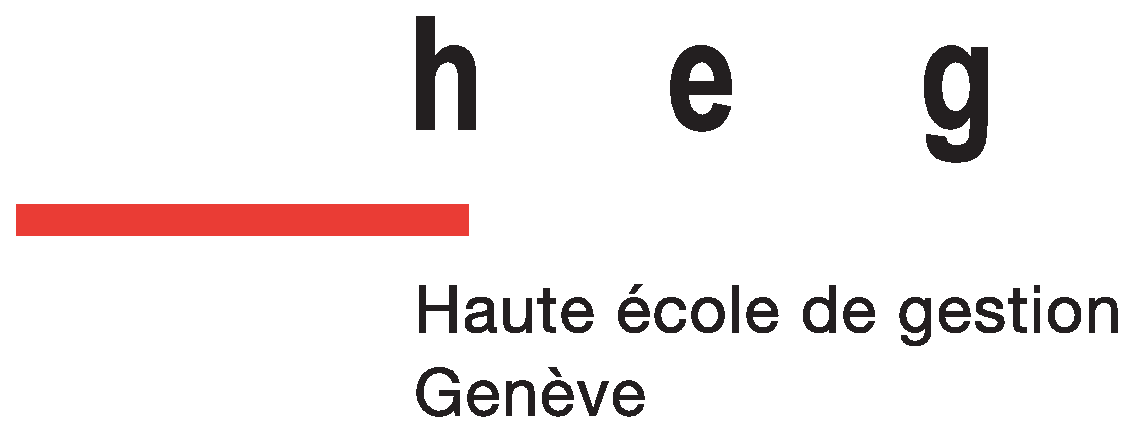
\includegraphics[width=4cm]{images/heg-logo.eps}
\end{flushleft}

\date{\vspace{0.2cm}}

\maketitle
\noindent \begin{center}

\includegraphics[width=2cm]{images/logo-mandant.png}				% Insérer le logo de votre mandant éventuel ici. Gérer la taille.
\par\end{center}{\Large \par}

\date{\vspace{4cm}
}

\noindent \begin{center}
\textbf{Travail de <Bachelor / Master> réalisé en vue de l’obtention du <Bachelor / Master>
HES}\\
par\textbf{\,}:
\par\end{center}
\noindent \begin{center}
\textbf{\Large <Votre prénom> \textsc{<Votre nom>}}
\par\end{center}{\Large \par}

\noindent \begin{center}
{\Large Conseiller au travail de <Bachelor / Master>\,:}\\
\textbf{\Large{} <Prénom> \textsc{<Nom>}, <titre de la personne>}
\par\end{center}{\Large \par}

\date{\vfill{}
}

\noindent \begin{center}
\textbf{\large Genève, \today{}}\\
\textbf{\large Haute École de Gestion de Genève (HEG-GE)}\\
\textbf{\large <filière>}
\par\end{center}{\large \par}

\vspace{2cm}


\begin{flushright}

\includegraphics[width=4cm]{images/hes-logo.eps}
\end{flushright}

\thispagestyle{empty}
\styleCenter

					% page de titre
	% ---------------------------------------------------------
% fichier includes/002-declaration.tex
% constitue la page de déclaration
% ---------------------------------------------------------

\newpage

\section*{Déclaration}		% l'étoile signifie qu'il s'agit d'un titre non numéroté

Ce travail de <Bachelor / Master> est réalisé dans le cadre de l’examen final de la Haute école de gestion de Genève, en vue de l’obtention du titre < … >.

L’étudiant a envoyé ce document par email à l'adresse remise par son conseiller au travail de <Bachelor / Master> pour analyse par le logiciel de détection de plagiat URKUND, selon la procédure détaillée à l’URL suivante : \url{http://www.urkund.fr/student_gorsahar.asp}.

L’étudiant accepte, le cas échéant, la clause de confidentialité. L'utilisation des conclusions et recommandations formulées dans le travail de <Bachelor / Master>, sans préjuger de leur valeur, n'engage ni la responsabilité de l'auteur, ni celle du conseiller au travail de <Bachelor / Master>, du juré et de la HEG. \bigskip{}


\enquote{J’atteste avoir réalisé seul le présent travail, sans avoir utilisé
des sources autres que celles citées dans la bibliographie.} \vspace{3cm}


\noindent \begin{flushright}
\begin{tabular}{l}
	\makeatletter		% permet d'utiliser la commande \@author
		Fait à <indiquez le lieu>, le \today{}\tabularnewline
		\@author\tabularnewline
		\tabularnewline
		<Votre signature>		% Supprimez cette ligne et remplacez-là par la signature
	\makeatother
\end{tabular}
\par\end{flushright}

\addcontentsline{toc}{section}{Déclaration}
\pagestyle{fancy}
				% déclaration
	\newpage

\section*{Remerciements}

Si vous avez des remerciements à formuler, à l’entreprise ou à toute autre personne qui a pu vous aider dans la réalisation du travail.


\addcontentsline{toc}{section}{Remerciements}

			% remerciements
	\newpage

\section*{Résumé}
  
Le résumé ne doit pas dépasser une page.

Il est rédigé dans le fichier \texttt{/includes/004-resume.tex}.

\bigskip

\textbf{\emph{Mots clés}}\emph{: <Mots; <clés> 
; <éventuels>}
\addcontentsline{toc}{section}{Résumé}
				% résumé et mots clés éventuels
	\newpage

\tableofcontents{}
%\addcontentsline{toc}{section}{Tables des matières}


\newpage

\begin{minipage}[t]{1\columnwidth}%

\renewcommand\listfigurename{Liste des tableaux}
\listoftables
\addcontentsline{toc}{section}{Liste des tableaux}

\renewcommand\listfigurename{Liste des figures}
\listoffigures
\addcontentsline{toc}{section}{Liste des figures}

\end{minipage}


\styleGauche

\cleardoublepage%cuz issue @preamble
\pagenumbering{arabic} %cuz issue @preamble
					% table des matières (table of content, toc)
	\section*{Introduction}

La mise en page du rapport de travail de Bachelor comprend une marge de 2,5 cm en haut et en bas, ainsi qu’à droite. À gauche, une marge de 3,5 cm est requise pour permettre la reliure.

La classe utilisée est \emph{article}, avec la police Arial 11 points et un espace entre les paragraphes au-dessus de 9 pt.

Le style « titre non numéroté centré » est utilisé pour Les titres suivants ne sont pas numérotés et sont centrés : déclaration, remerciements, résumé, liste des tableaux, liste des figures, bibliographie, annexes. Il faut utiliser l'étoile (*) pour l'indiquer.

Tous les éléments entourés de crochets < > doivent être modifiés ou effacés et tous les crochets doivent être supprimés.
N’oubliez pas de modifier le fichier \texttt{preambule/footerheader.tex} pour y inscrire le titre de votre travail de Bachelor ou de Master, ainsi que votre nom et votre prénom. Vous devez également le faire dans le fichier \texttt{includes/001-titre.tex} et \texttt{includes/002-declaration.txt}.

Pour les listes à puces, utilisez l'environnement \texttt{itemize} :

\begin{itemize}[itemsep=0pt]
	\item Énumération
	\item Énumération
	\begin{itemize}[itemsep=0pt]
		\item Énumération
		\item Énumération
	\end{itemize}
	\item Énumération
\end{itemize}

Pour les listes numérotées, utiliser de manière similaire l'environnement \texttt{enumerate}.

Lorsque vous commencer une nouvelle section de niveau 1, faites-le sur une nouvelle page, grâce à la commande \verb?\newpage?.

Faites attention à la cohérence dans la numérotation des pages. Avant l'introduction, les pages sont numérotées en chiffres romains. A partir de l'introduction, la numérotation reprend à 1 en chiffres arabes et doit être continue sur tout le document, y compris dans les annexes.

Pour les figures, insérez-les sur le modèle ci-dessous. N'oubliez pas la commande \verb?\caption{}? pour insérer la légende. Intégrer la source dans la légende.

\begin{figure}[H]
	\noindent \begin{centering}
	\caption{Titre de la figure}
	\bigskip{}
		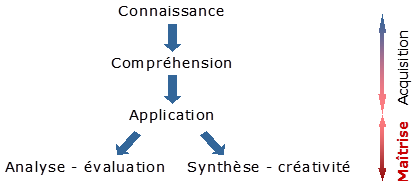
\includegraphics{images/image3.png}\bigskip{}
	\par\end{centering}
	\noindent \begin{raggedleft}
		Source: (Bertholet 2004, p. 22) % possibilité d'intégrer une référence avec BibTex
	\par\end{raggedleft}
\end{figure}

Procédez de manière similiare avec un tableau :

\begin{table}
	\noindent \begin{centering}
	\caption{Titre du tableau}
	\bigskip{}
		\begin{tabular}[h]{|c|c|m{0.2\textwidth}|}
			\hline
			Année & Ventes & Commandes \\
			\hline
			Truc & Truc & Truc \\
			\hline
			Truc & Truc & Truc \\
			\hline
		\end{tabular}
	\par\end{centering}
	\noindent \begin{raggedleft}
		Source: (Bertholet 2004, p. 22) % possibilité d'intégrer une référence avec BibTex
	\par\end{raggedleft}
\end{table}

\addcontentsline{toc}{section}{Introduction}
					% introduction
	% ----------------------------------------------
% fichier includes/1-chapitre1.tex
% premier chapitre
% ----------------------------------------------

\newpage

\section{Premier chapitre}

Il s'agit du fichier \texttt{1-chapitre1.tex} dans le répertoire \texttt{includes/}. Votre texte...

Votre texte...
				% premier chapitre
	% ------------------------------------------------
% fichier includes/3-chapitre2.tex
% deuxième chapitre
% ------------------------------------------------

\newpage

\section{Second chapitre}

Votre texte...

Votre texte...

\subsection{Titre de second niveau}

Votre texte...

Votre texte...

\subsection{Titre de second niveau}
 
Votre texte...
 
Votre texte...

\subsubsection{Titre de troisième niveau}
 
Votre texte...
 
Votre texte...

				% second chapitre
	% --------------------------------------
% fichier incluces/100-conclusion.tex
% conclusion
% le numéro du fichier à été choisi pour laisser la place. C'est arbitraire
% --------------------------------------


\newpage

\section{Conclusion}

Votre texte...

Votre texte...


				% conclusion
	% -----------------------------------------
% fichier includes/110-bibliographie.tex
% -----------------------------------------

\newpage

\printbibliography[title={Bibliographie}]


\addcontentsline{toc}{section}{Bibliographie}
			% bibliographie
	% -----------------------------------
% fichier includes/200-annexe1.tex
% -----------------------------------
\newpage
\section*{\centering{Annexe 1 : Titre de l'annexe}}

Votre texte ou le document mis en annexe. Le package \verb?pdfpages? permet d'intégrer des documents en format PDF.

Éviter de mettre deux annexes sur la même page. Insérez une nouvelle page, et indiquez le numéro de la nouvelle annexe et son titre.

\addcontentsline{toc}{section}{Annexe 1}
				% annexe 1



\end{document}
